% How we do it: Why we do it, What particular method we use and what logic architecture we use
\section{The methodological approach}
\label{MethodApproach}
%---What methodology we used---

We analyze the possibility of automatically transform a BPEL written process in a Java executable routine, with minimum ad-hoc developer’s intervention. Our final objective is to show the feasibility of a semi-automated transformation from a small business process orchestrated with BPEL to the Java language.
This section describes the steps we adopted to realize our goal. The following list summarizes the contents described in this Section.

\begin{itemize}
 \item Formalization of the languages involved in the transformation
 \item Description of the used approach: Programming vs Code Generation vs Model Driven Architecture).
 \item Choice of the specific MDA technique (M2M, M2T) that allows us to manipulate the BPEL input model and that is compatible with a ready to run code output.
 \item General outline of the methodological approach presented with an overview diagram.
\end{itemize}  

Once these steps have been accomplished, we focus on providing more details on how we carry out the transformation in the next section concerning the detailed architecture.
%\textbf{ALTRI DETTAGLI SONO NELLA SEZIONE DETAILED ARCHITECTURE ? }


\subsection{Languages involved in transformation} 
\label{sec:TransfDomain}
In our transformation we are dealing with BPEL, that is a generic language. Notwithstanding, since it has an XML-based concrete syntax, we deal with it as a DSL (Domain Specific Language) in order to apply M2M and M2T techniques. Java, on the other hand, is a multipurpose (textual) language.
Having to work with a model produced with a DSL means that we don't have to take care of the general constructs and ideas that are present in a generic language. The language is already skimmed to contain what is necessary to orchestrate business processes.
Concerning the output language, Java, it is not a DSL but a multipurpose language. Thus, it has no constraints on which kind of process or solution we could implement with it. %Most importantly, the fact the input model is produced in a DSL  

\subsection{The methodological approach}
\label{sec:ProgrammingVsMDE}
To realize the transformation, many possibilities arise; from a very specific, custom solution, to a more broad and abstract approach. The possibilities could be generalized in three main families: a manual ad-hoc programming solution, a code generation automation or a model driven architecture abstraction.
  \subsubsection{Ad-hoc Programming solution}
The programming solution would create an ad-hoc solution for our purpose. With this technique we would obtain a runnable, ready to deploy, solution. Though, as our aim is to provide a proof of concept for our approach, where the code is generated automatically, the focus on programming does not fit our needs.
  \subsubsection{Code Generation}
Code generation is aimed at automatizing the generation of code that would otherwise have to be written by hand. It concerns the creation of models/templates that will be later transformed in working code by an additional application. Although this solution might partially fit our need of an automated generation, we might have to create models/templates for many components, and we have to take into account a possible large amount of similar portions of code needed in different parts of the final application.  Thus, we need a solution that will rise of one more step the abstraction, where hierarchies and other software engineering concepts could be taken into consideration.
  
 \subsubsection{Model Driven Architecture (MDA) Abstraction}
The MDA aims, as well as the Code Generation automation, at the creation of models to be later transformed in runnable code (see Section \ref{MDA}). The difference lies in the fact that MDA permits to create an architecture where we could actually specify generic transformation strategies. For example, instead of creating a template for any BPEL construct, with MDA we could create a hierarchy of templates where similar BPEL constructs are sharing part of the code minimizing the quantity of hand written code at the price of a longer design phase.
\subsubsection{The proposed methodological approach}
Given the fact that our transformation has the purpose of showing the feasibility of a semi-automated transformation from BPEL to Java, we have to take into account that only a small part of the BPEL language can be considered. This implies that we have to propose a possibly expandable design for such a transformation, in case the BPEL subset would be enlarged. Last but not least, we have to keep an eye on possible future developments and improvements of the transformation itself. For these reasons, we decided to use a Model Driven Architecture methodology.

\subsection{Specific MDA approach: Template based M2T}
\label{sec:M2TApproach}
Once the MDA approach has been chosen, we have to choose which kind of model transformation we want to apply. As discussed in Section \ref{m2m&m2t}, there are two kinds of transformations: Model-to-Model and Model-to-Text. As we need a Java code output, the choice falls on the Model-to-Text type.This
Furthermore, Model-to-Text has itself two variants: visitor or template based. As discussed in Section \ref{m2m&m2t}, the visitor-based technique focus on traversing the input model's code and directly write text as output. While this technique would prove useful in case the translation could be carried out just as a sequence of steps, this is not true in the case of a BPEL to Java transformation. 
The structure of a BPEL model, which acts as an orchestrator of components, is very different from the Java object oriented application we wish to have as output.
This suggests we must be able to get values and parameters from several places of the input model and place them in several places of the output Java application. Thus, the template-based transformation fits our needs at best.

\subsection{Overview of the methodological approach}
\label{MethodologyOverview}
Once defined the methodology to be applied, we can sketch, as represented in Figure \ref{fig:TransformationApproach}, how the M2T technique is applied on our transformation.
\begin{figure}[ht]
  \begin{center}
    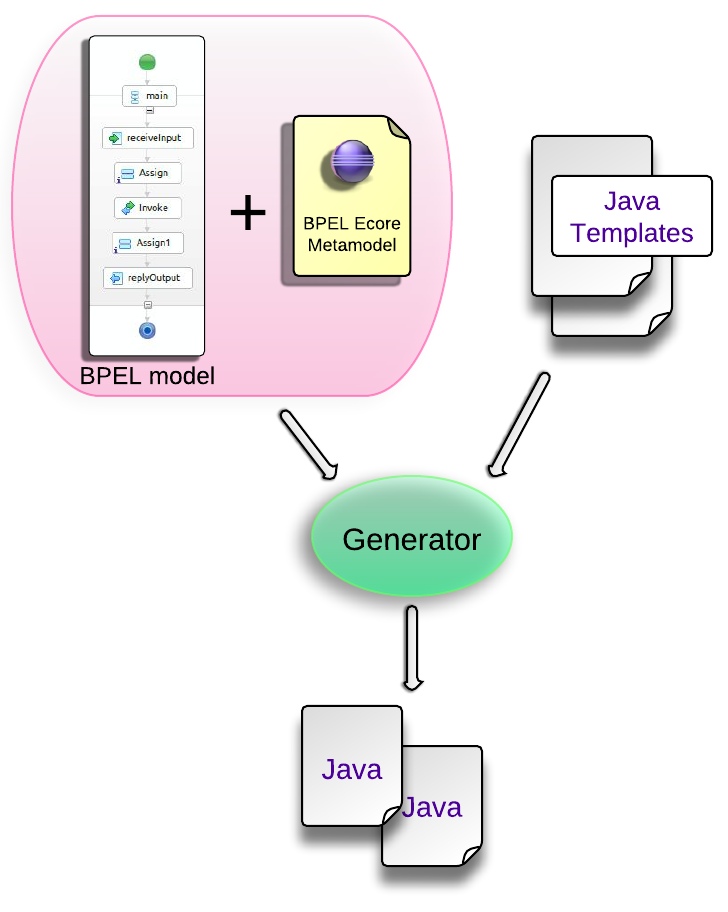
\includegraphics[scale=0.9]{pictures/TransformationApproach.png}
    \caption{The methodological transformation approach}
    \label{fig:TransformationApproach}
  \end{center}
\end{figure}
The inputs we have to provide in order to start the transformation are represented on the upper part of the picture. Namely, on the upper left there are represented the BPEL model of the process we want to transform in a Java application and the BPEL meta-model that will allow the parameterization of the process' elements. 
On the upper right there are the Java templates that define the structure of the final application. It is here that we define the hierarchy of objects and the inheritance strategies. In these templates we also determine where the dynamic elements taken from the BPEL model should be placed.  
In the middle, we have the Model-to-text generator. This component will mash the information from the parameterized input model with the Java templates to finally output a runnable Java application. This output application, written in Java code (represented at the bottom) should be able to mimic the orchestration logic played by the BPEL process given as input.  
Later in the report we also explain where and how the developer's intervention should be added on.




% %\lipsum[2]
% \hvFloat[
%  floatPos=!htb,
%  capWidth=h,
%  capPos=r,
%  capAngle=90,
%  objectAngle=90,
%  capVPos=c,
%  objectPos=c]{figure}{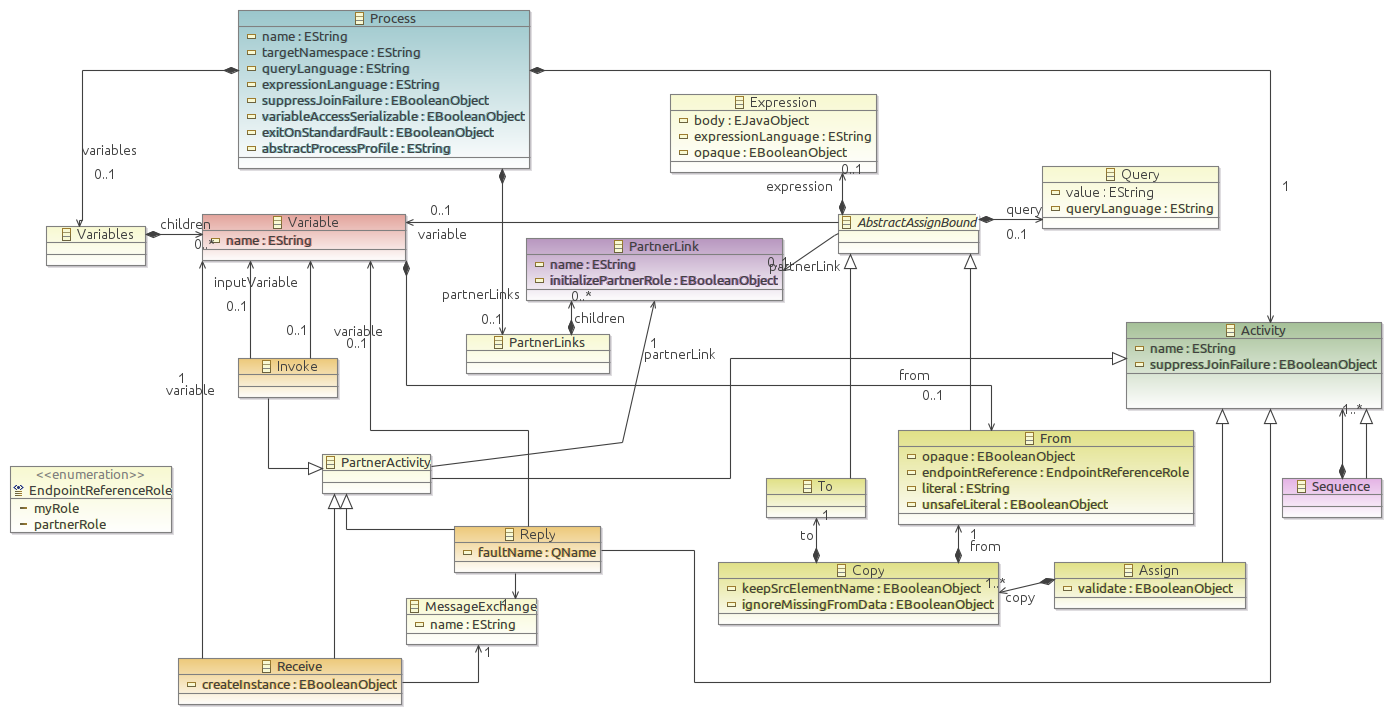
\includegraphics[scale=0.7]{pictures/SubSetBpel2.png}}%
% {Caption vertically centered right beside the float with a caption
% width of figure width and 
% \texttt{floatcapsep=5pt} (the default)}{fig:label}


%----------------------------------------------------


% \begin{multicols}{2}
% \begin{enumerate}
%     \item Basic activities:
%     \begin{itemize}
% 	\item \verb|<invoke>|
% 	\item \verb|<receive>|
% 	\item \verb|<reply>|
% 	\item \verb|<assign>|
% 	\end{itemize}
%     \item Structured activities: 
%     \begin{itemize}
% 	\item \verb|<sequence>|
%     \end{itemize}
%     \item  Elementary operations:
%     \begin{itemize}
% 	\item \verb|<copy>|
% 	\item \verb|<from>|
% 	\item \verb|<to>|
%     \end{itemize}
%     \item Static descriptive elements:
%     \begin{itemize}
% 	\item \verb|<process>|
% 	\item \verb|<partnerLink>|
% 	\item \verb|<variable>|
% 	\item \verb|<expression>|
%     \end{itemize}
% \end{enumerate}
% \end{multicols}